\documentclass[conference]{IEEEtran}
\usepackage{amsmath,amssymb,booktabs,graphicx,xcolor}
\usepackage[hidelinks]{hyperref}
\usepackage{url}
\usepackage{balance}
\usepackage{iftex}
\ifXeTeX
\usepackage{fontspec}
\setmainfont{texgyretermes-regular.otf}[BoldFont=texgyretermes-bold.otf,ItalicFont=texgyretermes-italic.otf,BoldItalicFont=texgyretermes-bolditalic.otf]
\setsansfont{texgyreheros-regular.otf}[BoldFont=texgyreheros-bold.otf,ItalicFont=texgyreheros-italic.otf]
\setmonofont{texgyrecursor-regular.otf}[BoldFont=texgyrecursor-bold.otf]
\fi
\definecolor{forest}{RGB}{32,75,64}
\title{Maintaining Source-Linked Evidence Views for Agent Memory}
\author{}
\begin{document}
\maketitle
\begin{abstract}
A memory service for an active agent must fit jointly useful evidence into context and detect when the source of a stored observation changes. We demonstrate SQLite views that maintain such evidence packets for tool traces and code edits. A prefix-aware dependency test recognized all 73,261 unchanged packets in 108,204 simulated source deletions. A faster conservative implementation delivered identical packets and reduced warm selection time by a factor of 5.16. On 2,000 ISETrace queries, learned evidence selection recovered every annotated source span in 83.07\% of cases versus 81.19\% for first-fit on the same native graph ranking. A separate checkpoint-selection protocol reproduced the gain. On 1,071 observed code edits, alignment inside editor-provided replacements preserved 323 complete packets versus 302 with range invalidation. Four interactive consoles let visitors remove a source, change a budget, follow an edit and inspect the evidence for each decision.

\end{abstract}

\section{Why maintain the evidence packet?}

A memory query may require an invocation and a later result in the same context. If a source disappears, must we rerun retrieval? In the demo, excluding one call replaces unit 11 with unit 19 at identical cost and coverage. Another exclusion needs no optimization. Even removal of an unselected candidate can affect the answer.

Wang et al.\ use execution provenance and relational graph models to retrieve supporting spans \cite{wang}. Bala examines which evidence survives packing \cite{bala}. Feng et al.\ study evidence needed in an observed coding-agent state \cite{feng}. MemTrace anchors immutable coding-agent traces to file, symbol and test identities and validates evidence before restoring it \cite{memtrace}. PACMI propagates validity changes through typed memory dependencies \cite{pacmi}. Qiu and Chen coordinate reads across stores using snapshots or epoch validation to deliver revision-consistent evidence \cite{readboundaries}. Retinraj studies how changed facts affect decisions in executable workflows \cite{changes}. Given a coherent snapshot and its exclusions, our question is whether its \emph{optimal budgeted packet} survives unchanged.

Yi et al.\ retain extra ranked tuples to reduce refills in materialized top-$k$ views \cite{topk}. Here a cumulative-cost prefix constrains a second optimization. TAPE demonstrates temporal graph memory for personal agents \cite{tape}. Our visitor inspects which provenance dependencies suffice to reuse this two-stage selection. Runtime work on evolving coding-agent state tracks which observations remain current \cite{execledger}. We additionally track when a valid observation can change the bounded answer.

\begin{figure}[t]
\centering
\setlength{\fboxsep}{4pt}
\begin{tabular}{@{}c@{}}
\fcolorbox{forest}{white}{\parbox{.88\columnwidth}{\centering \textbf{Public execution trace}\\Events, argument/output fields and character offsets}}\\
$\downarrow$\\
\fcolorbox{forest}{white}{\parbox{.88\columnwidth}{\centering \textbf{Read-only SQLite projection}\\Unit, source span, directed relation, cost, rank, utility}}\\
$\downarrow$\\
\fcolorbox{forest}{white}{\parbox{.88\columnwidth}{\centering \textbf{Materialized view and source dependencies}\\Protected prefix, packed suffix and prefix boundary}}\\
$\downarrow$\\
\fcolorbox{forest}{white}{\parbox{.88\columnwidth}{\centering \textbf{Live visitor controls}\\Exclude a source, inspect a unit, compare maintenance plans}}\\
\end{tabular}
\caption{Serving architecture. A separate evaluator receives the resulting unit IDs and compares their source intervals with a private annotation table on demand. The selection path has no access to that table or to the bodies of tool calls.}
\label{fig:system}
\end{figure}

\section{Selection and source dependencies}

\subsection{Materializing a view}
Candidate $i$ has cost $c_i\geq0$, utility $u_i$ and source intervals (event, field, half-open character offsets). Costs add across selected candidates. Evaluation merges overlapping intervals in source coordinates.

Let $B$ be the token budget and $T\leq B$ the prefix threshold. Protect the longest consecutive prefix $H$ costing at most $T$; the first candidate outside $H$ is its boundary. The first-fit comparator scans the entire ranking, admitting any candidate that still fits.

A gradient-boosted tree estimates candidate membership in the annotated evidence from graph and dense rank, type, cost, graph score and gap to the leader, and pool size. We fit it on 3,894 training queries weighted equally and transform its log-odds into positive utility with softplus. Joint sufficiency is measured separately on held-out queries.

Write $C=B-\sum_{i\in H} c_i$. On the remaining candidates the selector maximizes $\sum_i u_i x_i$ subject to $\sum_i c_i x_i\leq C$ and $x_i\in\{0,1\}$. A standard exact dynamic program updates the value at each integer capacity. Ties keep the existing solution. We return selected IDs in their original rank order. Threshold selection on 580 validation queries gave $T=1,024$ at $B=2,048$. Other thresholds trade a larger fixed prefix against additional freedom for the optimizer. The contribution here is a materialized packet with auditable source dependencies and maintenance rules.

\subsection{When can an exclusion change a packet?}
Let $P$ denote the stored packet and $D$ the set of candidate IDs removed by one or more source exclusions. Surviving candidates retain their order, costs and utilities. The budget, threshold and deterministic preference among tied solutions also stay fixed. Let $H'$ be the protected prefix recomputed on the remaining candidates.

\textbf{Reuse criterion.} The ordered packet is unchanged exactly when
\[
           D\cap P=\varnothing \quad\text{and}\quad H'\subseteq P.
\]
If a selected unit is removed, its ID cannot survive. If the new prefix contains a previously unselected unit, the new packet must contain that unit. For sufficiency, the first condition implies that all members of $H$ survive. Deletions can extend this prefix, so $H\subseteq H'$. By the second condition the old optimum contains every newly mandatory unit and remains feasible. Every packet feasible under the new requirement was already feasible before deletion. On these nested feasible families a previous optimum remains optimal, and the stable tie rule preserves its identity. Rank order of the surviving units is unchanged, giving equality of the ordered packets. The proof assumes exact comparisons and a stable tie order. A signed 64-bit implementation with fixed-point Q32 utilities reproduced all 10,000 original packets and all 108,204 deletion outcomes. The maximum tested utility sum was 13,789,213,370. Arbitrary floating-point summation orders do not inherit this guarantee.

A faster sufficient certificate indexes all sources of selected units and of the boundary. If an exclusion touches none of them, the old prefix survives and the suffix loses only unselected candidates. An index hit triggers recomputation, including some cases where the exact criterion would allow reuse.

For example, let $(B,T)=(8,4)$, costs $(3,3,1,5)$ and utilities $(1,1,3,10)$. Prefix $(0)$ and suffix $(3)$ fit. Removing unselected unit 1 forces prefix $(0,2)$ and leaves 4 tokens: unit 3 no longer fits.

\section{Implementation and visitor interaction}

SQLite stores query-local units, costs, utilities, source spans and typed edges. A parameterized anti-join excludes units attached to a removed source.

The trace projection contains 5,009 units and 10,789 typed edges for 40 hash-sampled queries from separate trajectories. ISETrace contains real tool executions for synthetic OS-agent tasks \cite{ise,wang}; we simulate source exclusions. A separate projection uses actual edits from Handoff Debt \cite{handoff}. Anonymized serving tuples and independent audit witnesses ship with the local consoles.

\begin{figure*}[t]
\centering
\begin{minipage}[t]{.48\textwidth}\vspace{0pt}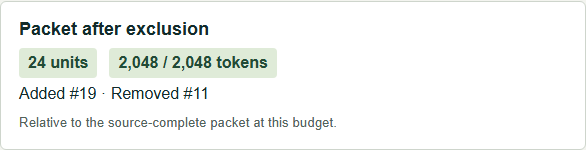
\includegraphics[width=\linewidth]{trace.png}\end{minipage}\hfill
\begin{minipage}[t]{.48\textwidth}\vspace{0pt}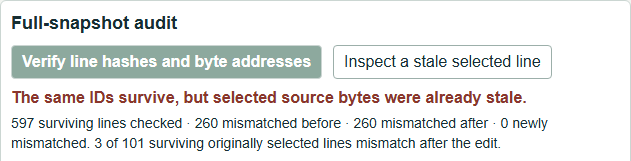
\includegraphics[width=\linewidth]{edit.png}\end{minipage}
\caption{Two running consoles. Left, excluding an execution source replaces unit 11 with unit 19 at the same cost. Right, a coding-agent edit retains the selected block IDs, yet the snapshot check detects incorrect line addresses in the original display. The audit operates separately from selection.}
\label{fig:ui}
\end{figure*}

\subsection{Visitor scenarios}
\textit{Change the trace evidence.} Select q02 and inspect a unit's source ranges. Exclude an unused source to reuse its packet, then exclude the selected source. Unit 19 replaces unit 11. Comparing the maintained result with full recomputation checks the ordered IDs. A separate evaluation control then shows that all 60 annotated characters remain covered.

\textit{Change the budget or boundary.} Reduce the token budget and inspect which supporting range drops out. In q07 an exclusion touches only the indexed prefix boundary. The conservative plan recomputes, while the exact test establishes that the packet survives.

\textit{Follow a real code edit.} A line shift preserves the first example's 315-byte packet. In the second, two of three blocks intersect the edit and only 74 of 507 bytes survive. The third retains all 14 IDs and 2,044 bytes, but the snapshot audit reveals three already incorrect addresses. We deliberately chose these examples to show distinct outcomes.

\textit{Reuse context from the edit itself.} The Edit Context console exposes the old and replacement line fingerprints. Choose the interior-lines example. Range invalidation drops both original blocks, matching the ends recovers one, and aligning equal runs restores both. The visitor changes the rule or byte budget and verifies the resulting coordinates against independently stored witnesses.

\textit{Inspect a withdrawn attribution.} The value-transfer console advances one tool group at a time. It shows when a second producer invalidates a unique value match, which direction flags change and how many stale flags an append-only policy would retain. Each step can be checked against a separately computed pair-table witness.

\section{Measurements and interpretation}
\subsection{Budgeted evidence recovery}
ISETrace provides 2,000 held-out queries over 1,207 trajectories. Its Full Support metric equals one when selected intervals jointly cover every annotated source interval. Both arms use the same candidate units, costs and five retrieval seeds. Retrieval intervals are paired 95\% crossed bootstraps over trajectories and seeds. In the first-fit control, skipped items leave their budget available for later candidates.

\begin{table}[t]
\caption{Evidence recovery under a 2,048-token cap. Values are means across five matched seeds on the complete test.}
\centering\small
\begin{tabular}{lrr}\toprule
Selector & Support (\%) & Tokens/query\\\midrule
Full R-GCN, strict prefix & 78.60 & 1,854.95\\
No adjacency, strict prefix & 79.21 & 1,850.31\\
Full R-GCN, first-fit & 80.44 & 2,039.97\\
No adjacency, first-fit & 81.19 & 2,039.83\\\midrule
Dense order + exact packing & 75.25 & 2,038.61\\
Graph rank-weighted packing & 80.37 & 2,036.40\\
Graph utility/cost greedy & 82.31 & 2,034.63\\
Same-ranker first-fit & 82.19 & 2,039.30\\
Prefix + exact packing & 82.60 & 2,039.12\\
No adjacency + learned packing & 83.07 & 2,039.12\\
\bottomrule\end{tabular}
\label{tab:retrieval}
\end{table}

Wang et al. report 77.33\% Full Support for the residual R-GCN in their main table \cite{wang}. Our controlled comparisons use local retraining of both native configurations. The full native relational graph model and its separately trained ablation without chunk adjacency are paired by seed, query, candidate set and cost. Our primary graph ordering with learned packing reaches 82.60\%, versus 82.19\% for its own first-fit (difference $+0.41$ points, crossed 95\% interval $[-0.23,1.08]$). Over six budgets from 256 to 8,192 tokens, normalized Full Support AUC is 70.992\% versus 70.565\% ($+0.427$ points, $[0.102,0.758]$).

Using the no-adjacency model's prefix and learned utility gained 1.88 points ($[0.76,3.07]$) against first-fit on the same ranking. This hybrid emerged after inspecting budget curves. Repeating training and choosing checkpoints by development Full Support instead of Recall@5 yielded 82.94\% versus 80.90\% ($+2.04$, $[0.71,3.40]$). Sorting the tail by absolute learned utility reached 82.98\% on these same weights. Exact optimization enables a well-defined view and reuse proof; its incremental retrieval benefit over this simple selector is uncertain. The live trace console uses the primary 82.60\% configuration.

At the halfway checkpoint we rebuilt graphs from truncated raw histories. On 901 questions in 657 trajectories with all evidence already present, our ranking with first-fit reached 84.73\%, dense first-fit 77.25\%, and the stronger native no-adjacency model 81.38\% ($+3.35$ points over native, $[1.40,5.35]$). All used approximately 2,014 tokens. Filtering completed native rankings to visible candidates gave 84.24\%, overstating the actual baseline by 2.86 points ($[1.59,4.24]$). Reciprocal rank fusion reached 85.50\% ($+0.78$ over our rank, $[-0.54,2.09]$). On all 2,000 questions, including unavailable evidence, our rank, the native comparator and their fusion attained 40.65\%, 39.01\% and 40.98\%, respectively. Query times are simulated.

What contributed beyond position and recency? Holding the training set, boosting model, E5 scores, token costs, event metadata and selector fixed, adding typed graph-degree features raised Full Support from 79.16\% to 83.57\% ($+4.42$ points, $[2.79,6.09]$). Adding cross-event relations to a reader that already had local relations gained 4.17 points ($[2.57,5.83]$). Local relations alone added 0.24 points to metadata ($[-0.60,1.12]$). Permuting the assignment of degree vectors within each role reduced support to 78.89\%. Within cross-event features, value flow alone reached 83.35\%, versus 79.47\% for links via a shared resource ($+3.88$ points, $[2.24,5.58]$). Two binary features indicating any incoming or outgoing value transfer still reached 82.91\%. A fixed online trigger after eight completed tool-call groups reproduced the feature gain on 649 eligible questions: 85.67\% versus 81.17\% ($+4.50$, $[2.92,6.14]$). Native no-adjacency reached 83.51\%; its paired difference from our full model included zero. On all 2,000 assignments, counting 94 unfired triggers as failures, the full and metadata-only models reached 29.79\% and 28.13\%. Questions in both schedules originated from completed traces.


\subsection{View maintenance on a live projection}
On 40 projections the portable reader reproduced every ordered packet; 36 had complete support. The conservative certificate reused packets for 2,041 of 2,528 independent source exclusions (80.74\%) and recomputed 487. All results matched fresh selection. Three recomputed packets had not changed.

Three interleaved repetitions gave 7,584 executions per plan. Full recomputation took $5.16\times$ as long as certificate-based serving (trajectory-bootstrap 95\% interval $[4.36,6.17]$). Median latency fell from 280.25 to 9.30 microseconds and p95 from 540.29 to 352.82 microseconds. Index setup cost 116 microseconds per query on average. These warm single-host measurements cover SQLite serving with precomputed model features. The portable interactive version implements the same selection in Python.

\balance
\begin{table}[t]
\caption{Exact reuse under independent hypothetical source exclusions. The final column counts additional reuse approvals beyond the fast boundary certificate.}
\centering\small
\begin{tabular}{rrrr}\toprule
Sources removed & Cases & Unchanged & Additional\\\midrule
1 & 2,528 & 2,044 & 3\\
2 & 97,676 & 68,336 & 232\\
3 & 4,000 & 1,991 & 12\\
8 & 4,000 & 890 & 17\\
\bottomrule\end{tabular}
\label{tab:exclusions}
\end{table}

Across 108,204 source-deletion sets (Table~\ref{tab:exclusions}), the exact criterion identified all 73,261 unchanged packets and certified 264 more reuses than the conservative index. Exhaustive checks of 20,204 deletion sets on 320 small synthetic pools also passed, including ties. These results assume fixed scores, costs, rank and budget. The timed speedup concerns the conservative single-source plan.

For value-transfer flags we also compared physical SQLite representations across 31,279 observed tool-group boundaries. Endpoint counts occupied 128 KiB, versus 208 KiB for weighted source--target pairs with a reverse index. The fastest pair-table scan took $1.18\times$ as long as endpoint maintenance with one full read per update ($[1.17,1.20]$), and $1.05\times$ with four ($[1.03,1.06]$). A stand-alone scan was faster for reads alone. Both plans reproduced every flag. Shared extraction of witness updates took 61.3 seconds and is excluded from these operator ratios.

\section{Serving memory during code edits}
We replayed 3,525 observed write attempts from Handoff Debt~\cite{handoff} on 37 issues across five Python repositories. Windows were selected around an observed read followed by a confirmed replacement. A separate integer view packs recent line blocks under a 2,048-byte cap. Whole-file invalidation permitted reuse in six of 2,820 attempts affecting a present path. Invalidation granularity and workload therefore matter to the benefit of caching.

A receipt locates the changed lines. We invalidate overlapping blocks and shift surviving addresses. A guard withholds displayed suffixes after clipping or coordinate discontinuities. Frozen on 24 issues, it retained 43,299 of 47,924 candidate lines on the other 13. Across 1,071 edits, range maintenance preserved 302 complete packets, versus 2 for file invalidation, 92 for symbol invalidation using Python syntax trees, and 287 for unique content matching against the new file. Issue-macro gains were 26.14 points over files ($[19.70,32.23]$), 17.92 over symbols ($[12.73,23.01]$) and 1.56 over content ($[-2.19,5.39]$). Content matching retained more individual bytes. All 25,912 surviving lines checked on edited paths matched their subsequent snapshots. 

An editor replacement also supplies two literal strings. We compare boundary-tagged line fingerprints, anchor their common ends and align unchanged interior runs within a bounded edit window. A block survives if every line maps to a consecutive equal line. Using just the common ends preserved 322 packets, and adding the interior alignment preserved 323 ($+1.97$ issue-macro points over range invalidation, $[1.02,3.03]$). All 29,713 mapped lines matched their snapshots. Across these operations the literals totalled 1.22 MB, versus 141.18 MB for pairs of complete file versions. A backend with version access can combine range validation with unique content lookup for intersecting blocks: it preserved 341 packets ($+4.52$ points over unique lookup alone, $[2.13,7.41]$).

Packet stability does not establish subsequent use. We followed requests until the next edit, termination or loss of observability. On this cohort 69 informative reads occurred in 54 observable episodes, with 889 right-censored windows. Range validation and local alignment supplied evidence beyond the edit receipt in the same 13 episodes. They fully covered 4 and 6 of these reads, respectively, when combined with the receipt. On a separate public SWE-agent run with Claude 4 Sonnet~\cite{swe-run}, we excluded all tasks shared with Handoff Debt. Across 265 eligible edits from 159 SWE-bench Verified issues, local alignment preserved 7 packets versus 5 for ranges ($+0.75$ issue-macro points, $[0.00,2.14]$). Source localization succeeded for 178 edits. This transfer is inconclusive. These observations concern trace replay. An independent coding-agent study also finds that estimating executed model work requires accounting for prefix-cache reuse \cite{physical}.

On 40 ISETrace projections we also replayed arrivals at the original message positions. Caching the optimal suffix for each capacity and updating it after new units gave exactly the full solution at all 2,336 steps and reduced selector time by $3.88\times$ ($[3.16,4.83]$) on one CPU. This separate operator study fixes costs, ranks and utilities throughout each replay; it excludes encoder and graph-scoring time. The visitor scenarios expose packet identity, source validity and the cost of maintaining each.

\section*{Acknowledgments}
OpenAI Codex assisted with the design and implementation of the methods in Sections II and III, experimental pipelines and analyses in Sections IV and V, preparation of the figures and demonstration, and drafting of the manuscript. Reported measurements were computed by the cited evaluation code and checked against persisted per-query or per-edit results.

\bibliographystyle{IEEEtran}
\bibliography{sources}
\end{document}
